\documentclass[journal]{IEEEtran}
\usepackage{amsmath,amssymb}
\usepackage{graphicx}
\usepackage{booktabs}
\usepackage{multirow}
\usepackage{array}
\usepackage{url}
\usepackage{cite}
\usepackage{xcolor}
\usepackage{tikz}
\usetikzlibrary{arrows.meta,positioning,shapes.geometric}
\usepackage{pgfplots}
\pgfplotsset{compat=1.18}
\usepackage{balance}

\title{UATimer: Lightweight Context-Aware Power Management for Heterogeneous IoT Systems}

\author{Geunsik Lim%
\thanks{G. Lim is with the Department of Electrical and Computer Engineering, Sungkyunkwan University, 2066 Seobu-ro, Jangan-gu, Suwon, Republic of Korea (e-mail: leemgs@g.skku.edu).}%
}

\begin{document}
\maketitle

\begin{abstract}
Energy-constrained Internet-of-Things (IoT) devices must enter low-power states aggressively without imposing unacceptable wake-up delay. Fixed inactivity timeouts are inexpensive but insensitive to changing activity, while predictive policies can add training, inference, and model-management overhead. This paper presents UATimer, a lightweight context-aware adaptive timer that updates an idle threshold from observed inter-event intervals and shifts energy--latency priorities using coarse application context. The framework runs in user space, uses standard timer and event interfaces, requires fewer than 500 lines of code and less than 1~KB of policy state, and does not require kernel modification. We evaluate the mechanism on a smartphone, a tablet, and an IoT sensor node using web browsing, video playback, on-device AI inference, AR/VR gaming, and periodic sensing workloads. Across the reported workload means, UATimer reduces energy by 20.5--37.5\% relative to the default baseline and by 7.9--16.7\% relative to a fixed-timeout policy while keeping average event delay below 50~ms. In the AR/VR workload, it reports a 0.5\% frame-drop rate and 1.2~ms jitter. Against a deliberately lightweight linear-regression predictor, UATimer yields similar energy values with a smaller policy footprint and no trained model. The results support UATimer as a deployable policy layer between static timeouts and heavier predictive power-management approaches.
\end{abstract}

\begin{IEEEkeywords}
Internet of Things, constrained devices, power management, energy efficiency, adaptive timer, context-aware systems, embedded systems.
\end{IEEEkeywords}

\section{Introduction}
\IEEEPARstart{B}{attery}-operated IoT and mobile-edge platforms increasingly execute interactive, sensing, communication, and inference workloads on the same device. Their energy budget is constrained not only by computation but also by repeated transitions among active, idle, and low-power states. A timeout that is too long wastes energy during idle intervals, whereas an overly aggressive timeout increases wake-up frequency and response delay. This tension is particularly important for systems that mix latency-sensitive tasks with long background idle periods.

Conventional operating-system power policies typically rely on fixed inactivity thresholds or coarse state machines. Such approaches are attractive because they are deterministic and inexpensive, but they can be poorly aligned with actual user behavior. Network-assisted duty cycling and IoT power-saving modes reduce active time, but their energy--latency behavior depends strongly on radio and paging configuration~\cite{michelinakis2021nbiot,eaps2022}. Mobile-system studies likewise show that idle and suspended states materially affect device energy use~\cite{carroll2010power}. These mechanisms do not directly solve the application-level question of how an interactive endpoint should adapt its suspend threshold to changing activity.

Recent work has explored context-aware mobile scheduling~\cite{lee2017cas}, predictive sleep scheduling~\cite{eaps2022}, and learning-based sleep policies for energy-constrained IoT systems~\cite{ko2025rass,ruiz2026wakeup}. However, the cost of adaptation can be non-trivial for resource-constrained devices. For small embedded platforms, even lightweight models introduce additional state, inference logic, and model-management complexity. This motivates a design point that is more adaptive than a fixed timeout but substantially simpler than a predictive learning system.

This paper develops such a design through a \emph{user-aware adaptive timer}. The framework observes inter-event idle periods, updates the timeout online, and modifies the energy--latency preference according to lightweight context. It is implemented as a user-space component that interoperates with existing Linux/Android power-management stacks and standard timer APIs. The design targets heterogeneous platforms ranging from smartphones and tablets to low-power IoT sensor nodes.

The main contributions are as follows:
\begin{itemize}
    \item We present a deployable user-space power-management layer that separates a portable suspend/resume mechanism from an online timeout policy, avoiding kernel modification and model training.
    \item We use a constant-state exponentially weighted idle-history update together with explicit context-dependent energy--delay priorities; the smoothing coefficient and objective weights are defined separately to avoid conflating temporal adaptation with policy preference.
    \item We describe an implementation with fewer than 500 lines of code and less than 1~KB of policy state, using PowerHAL-related callbacks on Android and \texttt{epoll}-based event hooks on Linux.
    \item We evaluate the mechanism across smartphone, tablet, and IoT-node platforms and five representative workloads, reporting energy, latency, and AR/VR quality indicators while explicitly identifying the limited IoT-platform breadth and five-run sample size.
    \item We compare against default OS behavior, fixed timeouts, and a deliberately lightweight linear-regression predictor. The comparison is positioned as evidence for a low-complexity operating point, not as a claim of superiority over modern TinyML or learning-based power managers.
\end{itemize}

The remainder of this paper is organized as follows. Section~II summarizes the design motivation and related approaches. Section~III presents the system architecture and adaptation algorithm. Section~IV describes the implementation. Section~V explains the experimental methodology, and Section~VI reports the results. Section~VII discusses implications, limitations, and extensions, followed by the conclusion in Section~VIII.

\section{Background and Design Motivation}
\subsection{Idle-State Power Management}
Mobile and IoT systems spend substantial time waiting for user input, network packets, sensor events, or periodic timers. Entering a deeper low-power state during these intervals can reduce energy consumption, but the transition itself carries latency and energy costs. Therefore, an effective policy must decide not only \emph{whether} to suspend but also \emph{when} to do so.

Fixed inactivity timeouts are commonly used because their behavior is predictable. Prior mobile work has shown that user context can expose idle intervals suitable for energy saving~\cite{pefkianakis2014idle,kim2012diapause}, while empirical NB-IoT studies show that power-state and paging configuration materially affect device energy consumption~\cite{michelinakis2021nbiot}. The drawback is that a fixed threshold cannot distinguish a bursty interactive session from a long unattended interval. A threshold chosen for responsiveness may remain too conservative at night or during sparse sensing, while a threshold optimized for energy saving can be disruptive during an AR/VR session.

\subsection{Learning-Based Policies}
Learning-based schedulers attempt to predict future idle intervals or workload states. In principle, prediction can reduce unnecessary transitions and increase energy savings. In practice, learning introduces new implementation requirements: feature extraction, model state, inference, training or retraining, and potentially hardware acceleration. These costs may be acceptable on high-end systems but less attractive for small IoT nodes or products that prioritize deterministic behavior and implementation simplicity.

The proposed framework is deliberately positioned between these two extremes. It uses recent observed idle intervals to adapt the timeout and allows simple context rules to adjust priorities. No training phase is required, and the policy state can be represented by a small number of scalar variables.

\subsection{Design Goals}
The framework was designed around five goals:
\begin{enumerate}
    \item \textbf{Low overhead:} negligible CPU and memory cost in comparison with the managed workload.
    \item \textbf{Responsiveness:} wake-up delay should remain suitable for interactive use.
    \item \textbf{Adaptivity:} the timeout should follow changing idle behavior rather than remaining fixed.
    \item \textbf{Portability:} the implementation should depend on generic user-space timer and event mechanisms rather than ISA-specific optimizations.
    \item \textbf{Deployability:} integration should not require kernel or driver modifications.
\end{enumerate}


\subsection{Relation to Existing Power-Management Techniques}
The proposed timer is intended to complement, rather than replace, established platform mechanisms. DVFS controls the energy cost of computation by changing voltage and frequency, while timer-based suspend/resume controls whether the platform should remain active during an idle interval. Network-side mechanisms such as duty cycling and predictive sleep scheduling reduce communication activity according to protocol behavior or learned delivery timing~\cite{eaps2022,ruiz2026wakeup}. UATimer operates at a different layer: it uses observed application and user activity to decide when a generic low-power transition is worthwhile. Consequently, the framework can coexist with processor-level DVFS and radio-specific power-saving mechanisms.

This distinction is also relevant to learning-based schedulers. A predictor attempts to estimate future behavior before making a transition decision. UATimer instead reacts to measured idle history and a small set of context labels. The latter cannot exploit complex latent correlations that might be available to a richer model, but it avoids training data, model distribution, inference dependencies, and retraining when the workload mix changes. For resource-constrained IoT nodes, eliminating these dependencies can be a meaningful engineering advantage even when the memory footprint of an individual model is small.

\begin{table}[t]
\caption{Positioning of UATimer Relative to Common Techniques}
\label{tab:positioning}
\centering
\scriptsize
\setlength{\tabcolsep}{2.2pt}
\begin{tabular}{p{0.18\columnwidth}p{0.21\columnwidth}p{0.20\columnwidth}p{0.27\columnwidth}}
\toprule
Technique & Primary control variable & Typical strength & Limitation addressed by UATimer \\
\midrule
Fixed timeout & Idle duration & Simplicity, determinism & No workload adaptation \\
DVFS/task mapping & Voltage/frequency, placement & Compute efficiency & Does not decide idle suspend timing \\
Protocol duty cycle & Radio/sampling schedule & Communication energy & Often schedule-driven \\
ML scheduler & Predicted idle/workload state & Rich adaptation & Training/inference complexity \\
UATimer & Adaptive idle threshold & Low-cost online adaptation & Coarse rather than learned context \\
\bottomrule
\end{tabular}
\end{table}

\subsection{IoT-Oriented Design Requirements}
An IoT-oriented policy must operate under constraints that are less visible on server-class systems. First, policy state should remain small enough to coexist with application buffers and protocol stacks on memory-constrained nodes. Second, adaptation should not require a persistent training pipeline, because many deployed devices have intermittent connectivity and long maintenance cycles. Third, the control path should be inspectable: a developer should be able to determine why a particular timeout was selected and to impose platform-specific minimum or maximum values. Finally, the same policy should remain usable when the endpoint changes from an interactive mobile device to a sensing node.

UATimer follows these requirements by maintaining only the current threshold, recent timing information, and a small amount of context state. The update in Eq.~\eqref{eq:update} is independent of the processor instruction set and does not assume a specific radio technology. The power-controller interface is therefore the platform-specific boundary: Android can map a transition to existing power-management services, Linux can use its suspend interfaces, and an MCU-class platform can map the same decision to its supported sleep state. This separation is central to the heterogeneous-system objective of the design.

\subsection{Parameterization Strategy}
The design uses representative energy-conservative, balanced, and latency-critical weight settings rather than a single universal configuration. This is appropriate because the acceptable latency penalty is application-dependent. A practical configuration process can therefore proceed in two stages. The platform first selects safe bounds $T_{min}$ and $T_{max}$ from its wake-up characteristics. The application then selects a context mode that determines the relative emphasis in Eq.~\eqref{eq:cost}. Within those limits, Eq.~\eqref{eq:update} continuously adapts to observed idle behavior.

This decomposition keeps parameter tuning interpretable. The smoothing factor $\lambda$ determines temporal responsiveness, the threshold bounds encode platform constraints, and $(w_E,w_D)$ encode application preference. None of these quantities requires a learned model. If future implementations introduce TinyML or statistical prediction, the predictor can be used to propose $t_{idle}$ while retaining the same bounded power-control interface.

\section{User-Aware Adaptive Timer Framework}
\subsection{System Architecture}
Fig.~\ref{fig:arch} shows the architecture. The \emph{User Interaction Monitor} captures user input and background events. The \emph{Timer Manager} maintains and updates the idle threshold. The \emph{Power Controller} invokes the underlying low-power transition and resumes the system on a new event.

\begin{figure}[t]
\centering
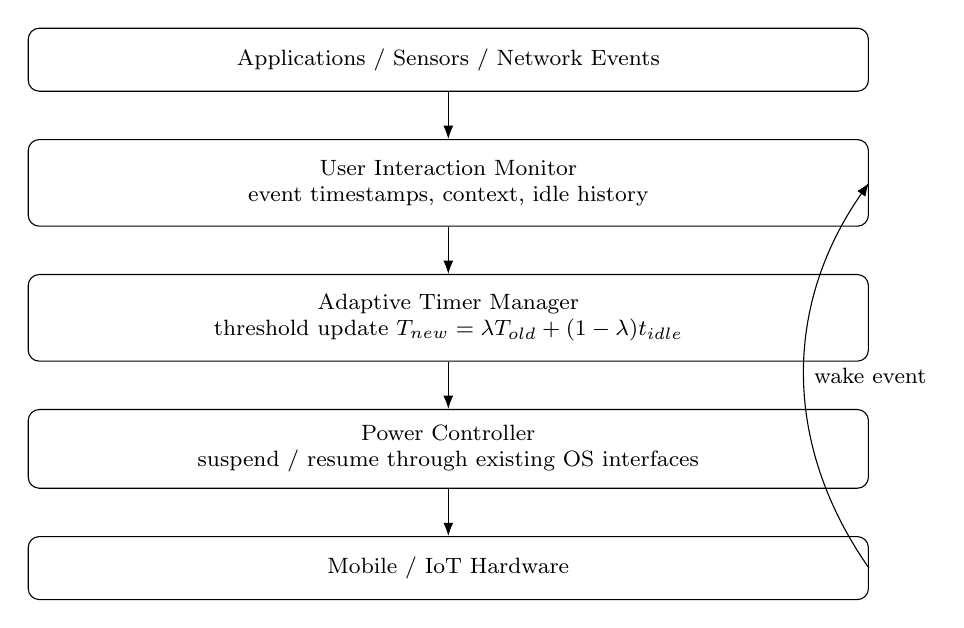
\begin{tikzpicture}[node distance=6mm, >=Latex, every node/.style={font=\footnotesize, align=center}]
\node[draw, rounded corners, minimum width=0.88\columnwidth, minimum height=8mm] (apps) {Applications / Sensors / Network Events};
\node[draw, rounded corners, below=of apps, minimum width=0.88\columnwidth, minimum height=11mm] (mon) {User Interaction Monitor\\event timestamps, context, idle history};
\node[draw, rounded corners, below=of mon, minimum width=0.88\columnwidth, minimum height=11mm] (timer) {Adaptive Timer Manager\\threshold update $T_{new}=\lambda T_{old}+(1-\lambda)t_{idle}$};
\node[draw, rounded corners, below=of timer, minimum width=0.88\columnwidth, minimum height=10mm] (power) {Power Controller\\suspend / resume through existing OS interfaces};
\node[draw, rounded corners, below=of power, minimum width=0.88\columnwidth, minimum height=8mm] (hw) {Mobile / IoT Hardware};
\draw[->] (apps) -- (mon);
\draw[->] (mon) -- (timer);
\draw[->] (timer) -- (power);
\draw[->] (power) -- (hw);
\draw[->, bend left=35] (hw.east) to node[right]{wake event} (mon.east);
\end{tikzpicture}
\caption{Architecture of the user-aware adaptive timer framework.}
\label{fig:arch}
\end{figure}

The framework does not alter the kernel scheduler or device drivers. Instead, it observes activity in user space and uses existing power-management interfaces. This separation minimizes integration effort and allows the same control logic to be reused across different processor architectures.

\subsection{Adaptive Timer Update}
Let $T$ denote the current idle threshold. When no activity occurs for $T$, the device enters a low-power state. When the next event occurs, the framework records the observed idle interval $t_{idle}$ and updates the threshold as
\begin{equation}
T_{new}=\lambda T_{old}+(1-\lambda)t_{idle},
\label{eq:update}
\end{equation}
where $0\leq\lambda<1$ is the temporal smoothing coefficient. A larger $\lambda$ produces slower changes and favors stability, whereas a smaller value responds more rapidly to recent observations.

The update can be implemented with only a few scalar variables. In contrast with a predictor that estimates a complete next-state distribution, the timer maintains a smoothed representation of recent idle behavior.

\subsection{Context-Aware Extension}
Observed idle duration alone cannot fully represent application requirements. The framework therefore permits context to modify the energy--responsiveness preference, consistent with context-aware mobile scheduling and QoS-aware power-management designs~\cite{lee2017cas,sang2024qos}. For example, an AR/VR application can increase the weight placed on delay, while night-time sensing can increase the emphasis on energy conservation.

We formalize this trade-off through
\begin{equation}
J(T)=w_E E(T)+w_D D(T),
\label{eq:cost}
\end{equation}
where $E(T)$ denotes energy consumption and $D(T)$ denotes average response delay under threshold $T$. The coefficients $w_E$ and $w_D$ reflect the active policy objective and are distinct from the temporal smoothing coefficient $\lambda$. Table~\ref{tab:weights} shows representative settings used to explain three operating modes.

\begin{table}[t]
\caption{Representative Energy--Delay Weight Settings}
\label{tab:weights}
\centering
\begin{tabular}{ccc}
\toprule
$w_E$ & $w_D$ & Priority mode \\
\midrule
0.8 & 0.2 & Energy-conservative \\
0.5 & 0.5 & Balanced \\
0.2 & 0.8 & Latency-critical \\
\bottomrule
\end{tabular}
\end{table}

The weighting mechanism is intentionally simple. It provides a way to react to coarse application context without requiring a learned policy.

\subsection{Algorithm}
Algorithm~\ref{alg:concept} summarizes the control flow in compact form.

\begin{figure}[t]
\small
\begin{verbatim}
on_event():
    now  = now_ms()
    idle = now - last_event
    last_event = now

    if context == ARVR:
        w_D += delta
        w_E -= delta
    else if context == NIGHT:
        w_E += delta
        w_D -= delta

    T = lambda*T + (1-lambda)*idle

main_loop():
    while true:
        if idle_ms() >= T:
            suspend()
        if event_available():
            resume_if_needed()
            on_event()
\end{verbatim}
\caption{Conceptual pseudocode of the adaptive timer.}
\label{alg:concept}
\end{figure}


\subsection{State-Machine Interpretation and Event Semantics}
The framework can also be viewed as a three-state controller with \emph{active}, \emph{idle-wait}, and \emph{low-power} states. After an event is serviced, the system enters the idle-wait state and arms the current threshold $T$. A new event arriving before expiry cancels the transition and produces a new idle observation. If the threshold expires, the Power Controller requests a low-power state. The next eligible user, sensor, or network event resumes the device and closes the current idle sample. This formulation separates \emph{policy} (how $T$ is selected) from \emph{mechanism} (how the platform enters or exits low power), which is useful for heterogeneous IoT systems whose suspend primitives differ across operating systems and microcontrollers.

To avoid pathological behavior, a practical deployment can constrain the adaptive threshold to a platform-defined interval
\begin{equation}
T_{min} \le T \le T_{max},
\label{eq:bounds}
\end{equation}
where $T_{min}$ protects latency-sensitive applications from excessively frequent transitions and $T_{max}$ limits idle energy waste. The implementation emphasizes lightweight adaptation rather than a learned transition policy; therefore, such bounds can be enforced with constant-time scalar operations and without changing the kernel interface.

\subsection{Convergence and Responsiveness of the Update Rule}
Equation~\eqref{eq:update} is an exponentially weighted update. For a stationary sequence with constant idle interval $t^*$, repeated application gives
\begin{equation}
T_k-t^*=\lambda^k(T_0-t^*),
\label{eq:convergence}
\end{equation}
so the threshold approaches the observed idle interval geometrically whenever $0\le\lambda<1$. This simple property clarifies the role of $\lambda$: larger values suppress short-term variation but require more events to follow a workload shift, while smaller values react faster but track transient bursts more closely. The implementation therefore exposes a direct and interpretable responsiveness knob rather than hiding adaptation inside model parameters.

For a non-stationary event stream, the same update can be interpreted as an exponentially weighted moving average of past idle intervals,
\begin{equation}
T_k=\lambda^kT_0+(1-\lambda)\sum_{i=0}^{k-1}\lambda^i t_{k-i},
\label{eq:ewma}
\end{equation}
which gives recent observations greater influence. This interpretation is important for IoT deployments because bursty user interaction, periodic sensing, and long unattended periods can occur on the same device. Context-aware changes to the energy--delay weights operate orthogonally to this temporal smoothing: $\lambda$ controls how quickly the timer follows history, while $(w_E,w_D)$ expresses the current application priority.

\subsection{Policy Complexity and Deployment Properties}
Table~\ref{tab:policycompare} summarizes the qualitative differences among the evaluated policies. The comparison is based on the implemented mechanisms rather than on additional performance measurements. The fixed timeout has the smallest control logic but cannot adapt. The linear-regression baseline adds prediction state and an inference path. UATimer retains constant-size scalar state and an $O(1)$ update per event while adapting online and accepting context input.

\begin{table}[t]
\caption{Qualitative Policy Characteristics}
\label{tab:policycompare}
\centering
\scriptsize
\begin{tabular}{p{0.20\columnwidth}cccc}
\toprule
Property & Baseline & Fixed & ML & UATimer \\
\midrule
Online adaptation & -- & No & Yes & Yes \\
Training required & -- & No & Yes & No \\
Context hook & OS dep. & No & Optional & Yes \\
Per-event update & OS dep. & $O(1)$ & inference & $O(1)$ \\
Kernel change & No & No & No & No \\
Policy state & OS dep. & scalar & coefficients & $<$1 KB \\
\bottomrule
\end{tabular}
\end{table}

\section{Implementation}
\subsection{User-Space Integration}
The implementation operates in user space and requires no kernel modification. On Android, the daemon registers PowerHAL-related callbacks to observe relevant activity and coordinate low-power transitions. On Linux, it uses \texttt{epoll}-based input hooks to detect events and a high-resolution timer to arm and disarm timeout decisions. Deployment changes are limited to user-space startup and manifest/init integration rather than kernel or driver patches.

The implementation size is below 500 lines of code, and the persistent policy state is below 1~KB. These properties are important for embedded deployment because they reduce the maintenance burden and avoid a model-management pipeline.

\subsection{Cross-Architecture Portability}
The control logic depends on timer APIs and user-space event hooks rather than processor-specific instructions. The implementation was evaluated primarily on ARM-based mobile platforms and additionally exercised on an Intel x86 Linux laptop and an ESP32-class RISC-V IoT board. This provides a portability check, not a full cross-architecture performance evaluation. It indicates that the control logic can be transferred when equivalent event and suspend/resume interfaces are available; the present dataset does not contain energy or latency measurements for the additional x86 and RISC-V systems.

\subsection{Lightweight ML Baseline}
For comparison, a linear-regression scheduler predicts the next idle interval from the previous three idle intervals and a bias term. The model is trained by least squares on $10^3$ samples and stores four scalar coefficients, requiring less than 64~B of model state. The reported per-event inference time is below 0.3~ms on a Cortex-A53 platform. This baseline was selected to represent a deliberately lightweight learning approach rather than a state-of-the-art neural or TinyML predictor. Consequently, the comparison supports only the claim that UATimer reaches a similar operating point to this specific predictor with simpler policy state; it must not be interpreted as a general comparison against learning-based power management.

\section{Experimental Methodology}
\subsection{Platforms}
The evaluation covers three representative device classes:
\begin{itemize}
    \item an Android smartphone based on a Qualcomm Snapdragon platform with a 4000~mAh battery,
    \item a tablet based on an ARM Cortex-A73 platform with a 6000~mAh battery, and
    \item a Cortex-M4 IoT sensor node powered by a coin-cell battery.
\end{itemize}
Energy on the mobile devices was measured using a Monsoon power monitor, while an external meter was used for the IoT node. Event latency was obtained from timestamp logging. Wi-Fi was enabled and display brightness was fixed at 50\% for the mobile-device experiments.

\subsection{Workloads}
Five workload classes were used:
\begin{itemize}
    \item \textbf{Web browsing:} intermittent touch input mixed with background network activity;
    \item \textbf{Video playback:} continuous decoding with relatively little user input;
    \item \textbf{AI inference:} long-running on-device DNN execution;
    \item \textbf{AR/VR gaming:} 60-Hz rendering with frequent sensor and interaction events; and
    \item \textbf{IoT sensing:} periodic sensor sampling and wireless transmission.
\end{itemize}

\subsection{Compared Policies}
Four policies were compared:
\begin{enumerate}
    \item \textbf{Baseline:} default OS behavior without additional timeout tuning;
    \item \textbf{Fixed timeout:} a static timeout representative of conventional idle policies;
    \item \textbf{ML scheduler:} the lightweight linear-regression predictor described above; and
    \item \textbf{Adaptive timer:} the proposed user-aware context-enhanced policy.
\end{enumerate}
Unless otherwise noted, the fixed-timeout configuration used 3~s for mobile workloads and 5~s for the IoT workload. Each experiment was repeated five times, and Table~\ref{tab:results} reports the arithmetic means available from those measurements. Because the archived dataset used to prepare this manuscript does not include the per-run samples, this version does not report reconstructed standard deviations, confidence intervals, or significance tests. This limitation is stated explicitly in Section~VII.


\section{Results}
\subsection{Energy and Latency}
Table~\ref{tab:results} summarizes the representative measurements. The proposed adaptive timer consistently reduces energy relative to the baseline while keeping average event delay below 50~ms.

\begin{table*}[t]
\caption{Representative Evaluation Results Across Workloads}
\label{tab:results}
\centering
\begin{tabular}{llrrrr}
\toprule
Workload & Policy & Energy (mJ) & Delay (ms) & Frame drop (\%) & Jitter (ms) \\
\midrule
Web Browsing & Baseline & 1200 & 30 & -- & -- \\
 & Fixed timeout & 900 & 50 & -- & -- \\
 & ML scheduler & 780 & 47 & -- & -- \\
 & Adaptive & \textbf{750} & 45 & -- & -- \\
\midrule
Video Playback & Baseline & 1800 & 25 & -- & -- \\
 & Fixed timeout & 1500 & 42 & -- & -- \\
 & ML scheduler & 1380 & 41 & -- & -- \\
 & Adaptive & \textbf{1350} & 40 & -- & -- \\
\midrule
AI Inference & Baseline & 2200 & 28 & -- & -- \\
 & Fixed timeout & 1900 & 40 & -- & -- \\
 & ML scheduler & 1780 & 39 & -- & -- \\
 & Adaptive & \textbf{1750} & 38 & -- & -- \\
\midrule
AR/VR Gaming & Baseline & 2500 & 20 & 2.5 & 3.0 \\
(60 Hz) & Fixed timeout & 2100 & 30 & 3.2 & 3.5 \\
 & ML scheduler & 1850 & 29 & 1.8 & 2.7 \\
 & Adaptive & \textbf{1800} & 28 & \textbf{0.5} & \textbf{1.2} \\
\midrule
IoT Sensing & Baseline & 400 & 12 & -- & -- \\
 & Fixed timeout & 320 & 18 & -- & -- \\
 & ML scheduler & 300 & 17 & -- & -- \\
 & Adaptive & \textbf{290} & 17 & -- & -- \\
\bottomrule
\end{tabular}
\end{table*}

Across the five workload classes, direct calculation from Table~\ref{tab:results} gives baseline-relative energy reductions of 20.5--37.5\% (mean 27.3\% across the five listed workload means). Relative to the fixed-timeout policy, the reduction is 7.9--16.7\%. The gap between the adaptive and ML schedulers is small in absolute energy (1.7--3.8\% lower for UATimer in the listed measurements), so the result should be interpreted primarily as a complexity/deployability trade-off rather than a large performance advantage over prediction.

\begin{figure}[t]
\centering
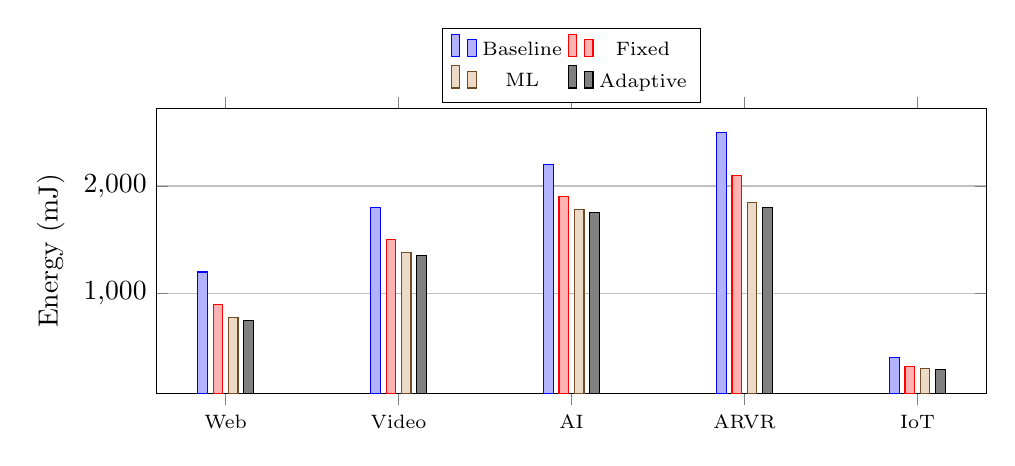
\begin{tikzpicture}
\begin{axis}[
    ybar,
    width=\columnwidth,
    height=5.2cm,
    ylabel={Energy (mJ)},
    symbolic x coords={Web,Video,AI,ARVR,IoT},
    xtick=data,
    x tick label style={font=\scriptsize},
    ymajorgrids=true,
    legend style={font=\scriptsize, at={(0.5,1.02)}, anchor=south, legend columns=2},
    bar width=3.5pt
]
\addplot coordinates {(Web,1200) (Video,1800) (AI,2200) (ARVR,2500) (IoT,400)};
\addplot coordinates {(Web,900) (Video,1500) (AI,1900) (ARVR,2100) (IoT,320)};
\addplot coordinates {(Web,780) (Video,1380) (AI,1780) (ARVR,1850) (IoT,300)};
\addplot coordinates {(Web,750) (Video,1350) (AI,1750) (ARVR,1800) (IoT,290)};
\legend{Baseline,Fixed,ML,Adaptive}
\end{axis}
\end{tikzpicture}
\caption{Energy consumption for the evaluated workloads.}
\label{fig:energy}
\end{figure}

\begin{figure}[t]
\centering
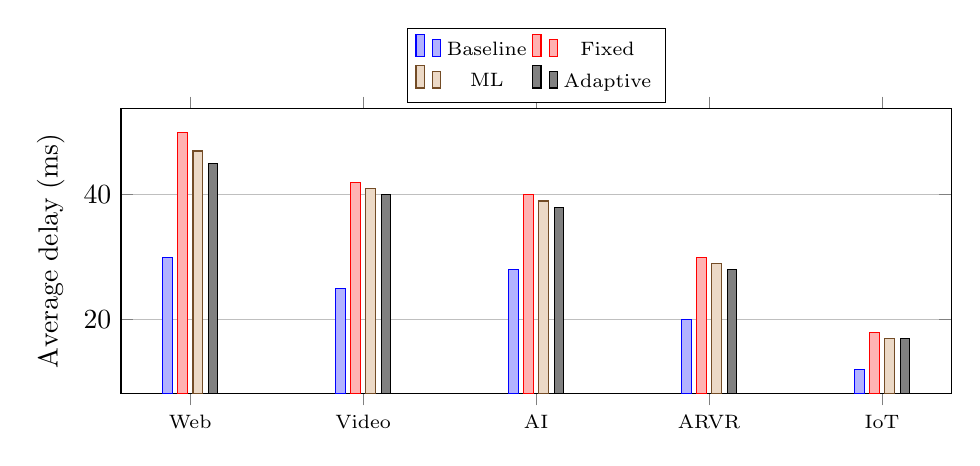
\begin{tikzpicture}
\begin{axis}[
    ybar,
    width=\columnwidth,
    height=5.2cm,
    ylabel={Average delay (ms)},
    symbolic x coords={Web,Video,AI,ARVR,IoT},
    xtick=data,
    x tick label style={font=\scriptsize},
    ymajorgrids=true,
    legend style={font=\scriptsize, at={(0.5,1.02)}, anchor=south, legend columns=2},
    bar width=3.5pt
]
\addplot coordinates {(Web,30) (Video,25) (AI,28) (ARVR,20) (IoT,12)};
\addplot coordinates {(Web,50) (Video,42) (AI,40) (ARVR,30) (IoT,18)};
\addplot coordinates {(Web,47) (Video,41) (AI,39) (ARVR,29) (IoT,17)};
\addplot coordinates {(Web,45) (Video,40) (AI,38) (ARVR,28) (IoT,17)};
\legend{Baseline,Fixed,ML,Adaptive}
\end{axis}
\end{tikzpicture}
\caption{Average event latency for the evaluated workloads.}
\label{fig:latency}
\end{figure}

\subsection{AR/VR Quality of Experience}
The AR/VR workload illustrates the need to avoid overly aggressive energy saving. The fixed-timeout policy reduces energy but increases frame drops to 3.2\% and jitter to 3.5~ms. The adaptive policy reduces energy from 2500~mJ to 1800~mJ while reporting only 0.5\% frame drops and 1.2~ms jitter. These measurements indicate that context-dependent weighting can preserve interactive quality while still exploiting idle opportunities.


\subsection{Comparison With the Lightweight ML Baseline}
The adaptive timer slightly outperforms the linear-regression scheduler in the reported energy measurements while exhibiting similar latency. The main distinction is implementation complexity: the adaptive method requires only scalar state and a deterministic update rule, whereas the learning baseline requires a feature representation, trained coefficients, and inference logic. Although the chosen ML baseline is intentionally lightweight, the comparison demonstrates that a simple adaptive mechanism can capture much of the available benefit for the evaluated workloads.


\subsection{Workload-Level Energy Reduction Derived From the Measurements}
To make the workload dependence more explicit, Table~\ref{tab:derived} reports reductions computed directly from the energy values in Table~\ref{tab:results}. These percentages are arithmetic transformations of the reported measurements and do not represent additional experimental runs. Relative to the default baseline, the computed reduction is 20.5--37.5\%; relative to the fixed-timeout policy, UATimer reduces measured energy by approximately 7.9--16.7\% across the five workloads. Relative to the lightweight ML scheduler, the additional reduction is smaller, approximately 1.7--3.8\%, which supports the observation that a low-complexity adaptive rule captures much of the benefit available to the selected predictor.

\begin{table}[t]
\caption{Energy Reduction Computed From Table~\ref{tab:results}}
\label{tab:derived}
\centering
\begin{tabular}{lrrr}
\toprule
Workload & vs. Baseline & vs. Fixed & vs. ML \\
 & (\%) & (\%) & (\%) \\
\midrule
Web browsing & 37.5 & 16.7 & 3.8 \\
Video playback & 25.0 & 10.0 & 2.2 \\
AI inference & 20.5 & 7.9 & 1.7 \\
AR/VR gaming & 28.0 & 14.3 & 2.7 \\
IoT sensing & 27.5 & 9.4 & 3.3 \\
\bottomrule
\end{tabular}
\end{table}

The absolute measurements also show that the benefit is not tied to a single workload class. The adaptive policy has the lowest reported energy value in every row group of Table~\ref{tab:results}. At the same time, its latency remains close to that of the ML scheduler, and in the AR/VR case the frame-drop and jitter values are lower than those of the other evaluated policies. Because the experiment reports only five repetitions per condition and per-run samples are not available in the archived dataset, these workload-level comparisons should be interpreted as representative mean differences rather than universal effect sizes.

\subsection{Energy--Latency Operating Point}
The measurements illustrate why power management should be treated as a multi-objective problem. The baseline generally has the lowest event delay but consumes more energy, while fixed timeouts reduce energy at the cost of larger delay. UATimer occupies an intermediate operating point: it gives up some baseline responsiveness to gain energy efficiency, but its observed delay remains below 50~ms for all evaluated workloads. For IoT deployments, this operating point can be shifted by changing context weights rather than replacing the control mechanism.

The AR/VR case is particularly informative. A purely energy-oriented policy can enter low-power states at times that disturb a 60-Hz rendering pipeline. By assigning greater weight to delay in latency-critical context, the timer can remain conservative while the application is active and become more aggressive when the context changes. Conversely, periodic sensing can tolerate longer thresholds and place more weight on energy conservation. The same runtime therefore supports heterogeneous device roles without maintaining a separate predictor for each workload class.

\subsection{Failure Modes and Safe Integration}
A deployable timer policy must account for cases in which suspending is undesirable even if the observed idle interval is long. Examples include non-deferrable background operations, protocol-critical communication windows, or device-specific transitions whose wake cost is high. The architecture addresses this at the integration boundary: platform or application context can inhibit a transition, select a latency-critical mode, or constrain $T$ through Eq.~\eqref{eq:bounds}. In this sense, UATimer is designed as a policy layer that complements rather than replaces existing platform safety and power-management controls.

The user-space placement also limits the failure domain. If the daemon is disabled or cannot obtain the required event hooks, the underlying OS policy remains available. This property is useful during staged deployment because the adaptive component can be enabled per product or workload without introducing an ISA-specific kernel patch. The trade-off is that user-space observation may not expose every device-level event; deeper component coordination would require additional platform interfaces.

\subsection{Validity Considerations}
Three considerations bound the interpretation of the present evaluation. \emph{Internal validity} depends on stable measurement conditions; Wi-Fi state and display brightness were fixed and each experiment was repeated five times, but uncontrolled background activity can still affect mobile energy measurements. \emph{Construct validity} is limited by the chosen metrics: total energy and average event latency capture the primary trade-off, while component-level residency, tail latency, and battery-lifetime projections are not reported. \emph{External validity} is limited by the three principal evaluation platforms, even though the user-space daemon was additionally exercised on x86 Linux and an ESP32-class RISC-V board. These considerations motivate broader measurements but do not change the reported means.


\subsection{Evidence Boundaries and Claims Supported by the Present Data}
The available measurements support four bounded conclusions. First, the adaptive policy has the lowest listed energy mean among the four evaluated policies for each of the five workloads. Second, average event delay for the adaptive policy remains below 50~ms in all listed workloads. Third, the reported AR/VR measurements show lower frame-drop and jitter values for the adaptive policy than for the three comparison policies. Fourth, the implementation is described as a small user-space component without kernel modification. The present data do \emph{not} establish superiority over modern TinyML policies, statistical significance across a large sample, radio-specific IoT energy behavior, or general cross-architecture energy gains. We state these boundaries explicitly to keep the claims aligned with the available measurements.

\section{Discussion}
\subsection{Why the Method Helps}
The main benefit of the framework is not the timer itself but the continual alignment of timeout duration with observed behavior. A fixed timeout assumes a stationary environment, while interactive systems are inherently non-stationary. Web activity alternates between bursts and pauses, sensing workloads can become sparse, and latency-sensitive applications can temporarily dominate the system. The exponential update in~\eqref{eq:update} allows the threshold to follow these changes without a separate prediction model.

\subsection{Workload Dependence}
The magnitude of the gain depends on the availability of idle intervals. Video playback creates a relatively continuous decode pipeline and therefore provides fewer opportunities for suspend/resume optimization. More generally, prior measurements show that the energy impact of power-state decisions is highly workload- and interface-dependent~\cite{carroll2010power,michelinakis2021nbiot}. In contrast, web browsing and periodic sensing contain more exploitable idle gaps. This explains why the margin between the ML and adaptive schemes is narrow in some workloads: once the available idle opportunities are captured, additional prediction complexity has limited room to improve total energy.

\subsection{Practical Deployment}
A key property is that deployment does not require kernel patches. In production environments, kernel modifications can increase validation cost and complicate updates across device variants. A user-space approach can be deployed selectively, disabled when necessary, and updated independently of low-level drivers. The resulting design is therefore suitable for experimental integration in mobile-edge and IoT products where maintainability is as important as algorithmic efficiency.

\subsection{Limitations}
The current evaluation has several limitations. First, the device set is representative rather than exhaustive, and only one principal IoT sensing platform contributes quantitative results. Second, the learning comparison uses a simple linear-regression model; stronger TinyML predictors would provide a more demanding baseline. Third, the present results focus on device-level energy and event latency and do not provide a component-level breakdown across CPU, GPU, radio, display, and memory. Fourth, only five repetitions were performed per condition, and the archived dataset available for this manuscript does not include per-run samples for retrospective uncertainty analysis. Finally, the context policy is rule-based and depends on manually defined application classes.

These limitations identify the highest-priority validation work for a subsequent experimental revision: evaluation on additional MCU and RISC-V boards, radio-specific experiments, battery-lifetime measurements, stronger TinyML baselines, component-level energy accounting, and a larger number of independent repetitions. Such extensions would strengthen generality without changing the core design.

\subsection{Reproducibility}
The implementation and evaluation scripts will be archived with the project repository at \url{https://github.com/leemgs/uatimer}. Reproducibility is particularly important for lightweight power-management mechanisms because small changes in timeout parameters, device state, and workload timing can affect measured energy savings.

\section{Conclusion}
This paper presented a user-aware adaptive timer framework for energy-efficient and responsive power management in heterogeneous IoT and mobile-edge systems. The framework dynamically updates the idle threshold from observed activity, uses lightweight context to shift energy--latency priorities, and operates entirely in user space without kernel modification. The implementation requires fewer than 500 lines of code and less than 1~KB of state. Across the reported browsing, video, AI, AR/VR, and sensing measurements, the adaptive mechanism reduces energy by 20.5--37.5\% relative to the default baseline and 7.9--16.7\% relative to the fixed-timeout policy while maintaining average event latency below 50~ms. It also reports favorable AR/VR quality indicators and energy values close to the deliberately lightweight linear-regression baseline, with simpler policy state. These characteristics make the design a practical middle ground between static timeout policies and heavier predictive schedulers for resource-constrained and interactive IoT platforms.

Future work will evaluate larger device populations, additional wireless protocols and edge workloads, stronger TinyML baselines, component-level energy behavior, and more independent repetitions. Another direction is joint management of CPU, GPU, display, and radio power states while preserving the same low-overhead user-space design principle.

\section*{Acknowledgment}
OpenAI ChatGPT was used to assist with drafting and restructuring portions of the Introduction, Background, Discussion, and language throughout the manuscript. The author reviewed and edited the generated text and takes responsibility for the final content. The AI system was not used to generate, alter, or fabricate experimental measurements or reported results.

\balance
\begin{thebibliography}{10}
\bibitem{carroll2010power} A. Carroll and G. Heiser, ``An analysis of power consumption in a smartphone,'' in \emph{Proc. USENIX Annu. Tech. Conf. (USENIX ATC)}, 2010.
\bibitem{kim2012diapause} Y. Kim and J. Kim, ``Personalized Diapause: Reducing radio energy consumption of smartphones by network-context aware dormancy predictions,'' in \emph{Proc. Workshop Power-Aware Computing and Systems (HotPower)}, 2012.
\bibitem{pefkianakis2014idle} I. Pefkianakis, J. Chandrashekar, and H. Lundgren, ``User-driven idle energy save for 802.11x mobile devices,'' in \emph{Proc. IEEE Int. Conf. Mobile Ad Hoc Sensor Syst. (MASS)}, 2014, pp. 282--290, doi: 10.1109/MASS.2014.50.
\bibitem{lee2017cas} J. Lee, K. Lee, E. Jeong, J. Jo, and N. B. Shroff, ``CAS: Context-aware background application scheduling in interactive mobile systems,'' \emph{IEEE J. Sel. Areas Commun.}, vol. 35, no. 5, pp. 1013--1029, May 2017, doi: 10.1109/JSAC.2017.2676918.
\bibitem{michelinakis2021nbiot} F. Michelinakis, A. S. Al-Selwi, M. Capuzzo, A. Zanella, K. Mahmood, and A. Elmokashfi, ``Dissecting energy consumption of NB-IoT devices empirically,'' \emph{IEEE Internet Things J.}, vol. 8, no. 2, pp. 1224--1242, Jan. 2021, doi: 10.1109/JIOT.2020.3013949.
\bibitem{eaps2022} J. Sheth, C. Miremadi, A. Dezfouli, and B. Dezfouli, ``EAPS: Edge-assisted predictive sleep scheduling for 802.11 IoT stations,'' \emph{IEEE Syst. J.}, vol. 16, no. 1, pp. 591--602, Mar. 2022, doi: 10.1109/JSYST.2021.3063922.
\bibitem{safaei2021elite} B. Safaei, A. M. Hosseini Monazzah, and A. Ejlali, ``ELITE: An elaborated cross-layer RPL objective function to achieve energy efficiency in Internet-of-Things devices,'' \emph{IEEE Internet Things J.}, vol. 8, no. 2, pp. 1169--1182, Jan. 2021, doi: 10.1109/JIOT.2020.3011968.
\bibitem{ko2025rass} H. Ko, H. Choi, and S. Pack, ``Restoration-aware sleep scheduling framework in energy harvesting Internet of Things: A deep reinforcement learning approach,'' \emph{IEEE Trans. Sustainable Comput.}, vol. 10, no. 1, pp. 190--198, Jan./Feb. 2025, doi: 10.1109/TSUSC.2024.3442918.
\bibitem{sang2024qos} Q. Sang, J. Yan, R. Xie, C. Hu, K. Suo, and D. Cheng, ``QoS-aware power management via scheduling and governing co-optimization on mobile devices,'' \emph{IEEE Trans. Mobile Comput.}, vol. 23, no. 12, pp. 13654--13669, Dec. 2024, doi: 10.1109/TMC.2024.3438267.
\bibitem{ruiz2026wakeup} D. E. Ruiz-Guirola, S. Montejo-Sanchez, I. Leyva-Mayorga, Z. Han, P. Popovski, and O. L. A. Lopez, ``Energy management and wakeup for IoT networks powered by energy harvesting,'' \emph{IEEE Internet Things J.}, vol. 13, no. 9, pp. 18574--18591, May 2026, doi: 10.1109/JIOT.2026.3664201.
\end{thebibliography}

\end{document}
